%%%%%%%%%%%%%%%%%%%%%%%%%%%%%%%%%%%%%%%%%
% Beamer Presentation
% LaTeX Template
% Version 1.0 (10/11/12)
%
% This template has been downloaded from:
% http://www.LaTeXTemplates.com
%
% License:
% CC BY-NC-SA 3.0 (http://creativecommons.org/licenses/by-nc-sa/3.0/)
%
%%%%%%%%%%%%%%%%%%%%%%%%%%%%%%%%%%%%%%%%%

%-------------------------------------------------------------------------------
%	PACKAGES AND THEMES
%-------------------------------------------------------------------------------

\documentclass{beamer}
\usepackage{xcolor}
\usepackage{graphicx}
\usepackage{tikz}
\usepackage{listings}
\usepackage{multicol}

\DeclareMathOperator{\diag}{diag}

\definecolor{applegreen}{rgb}{0.55, 0.71, 0.0}
\definecolor{blue(ncs)}{rgb}{0.0, 0.45, 0.60}
\definecolor{burgundy}{rgb}{0.5, 0.0, 0.13}

\definecolor{cadet}{rgb}{0.33, 0.41, 0.47}
\definecolor{airforceblue}{rgb}{0.36, 0.54, 0.66}

\mode<presentation> {

\usetheme{CambridgeUS}

\usecolortheme{wolverine}

\definecolor{gold}{HTML}{D4A017}
\definecolor{darkgold}{HTML}{B7950B}

\setbeamercolor{palette primary}{bg=cadet,fg=white}
\setbeamercolor{palette secondary}{bg=airforceblue,fg=white}
\setbeamercolor{palette tertiary}{bg=black,fg=white}
\setbeamercolor{palette quaternary}{bg=cadet,fg=white}

\setbeamercolor{frametitle}{bg=airforceblue,fg=white}

\setbeamercolor{section number projected}{bg=black,fg=cadet}
\setbeamercolor{item}{fg=black,bg=cadet}

\setbeamertemplate{page number in head/foot}[framenumber]

\lstset{basicstyle=\ttfamily\footnotesize,breaklines=true}
}



\lstdefinestyle{colouredC}{ 
  commentstyle=\color[gray]{0.4},
  keywordstyle=\bfseries,
  keywordstyle=[2]\color[rgb]{0.75, 0, 0},
  keywordstyle=[3]\color[rgb]{0, 0.5, 0},
  keywordstyle=[4]\color[rgb]{0, 0.5, 0},
  keywordstyle=[5]\color[rgb]{0, 0, 0.75},
  numberstyle=\tiny\color{mGray},
  stringstyle=\color[rgb]{0, 0, 0.5},
  basicstyle=\ttfamily,
  language=C,
  morekeywords=[3]{CeedInt, CeedScalar},
}

\lstdefinestyle{boxedC}{
  style=colouredC,
  numbers=left,
  firstnumber=auto,
  numberblanklines=true,
  frame=trbL,
  numberstyle=\tiny,
  frame=leftline,
  numbersep=7pt,
  framesep=5pt,
  framerule=10pt,
  xleftmargin=15pt,
  backgroundcolor=\color[gray]{0.97},
  rulecolor=\color[gray]{0.90}%
}

\usepackage{graphicx} % Allows including images
\usepackage{booktabs} % Allows the use of \toprule, \midrule and \bottomrule in tables

\newcommand{\mycomment}[1]{}

%----------------------------------------------------------------------------------------
%	TITLE PAGE
%----------------------------------------------------------------------------------------

\title[Ratel]{Ratel -  New Foundations of Computational Mechanics for the Exascale Era
} % The short title appears at the bottom of every slide, the full title is only on the title page

\author{Jeremy L Thompson} % Your name
\institute[CU Boulder] % Your institution as it will appear on the bottom of every slide, may be shorthand to save space
{University of Colorado Boulder \\ % Your institution for the title page
\medskip
\textit{jeremy@jeremylt.org} % Your email address
}
\date{1 May 2025} % Date, can be changed to a custom date

\begin{document}

\begin{frame}
\titlepage % Print the title page as the first slide
\end{frame}

%------------------------------------------------

\begin{frame}
\begin{center}
\frametitle{Interrupt Me!}

Please interrupt with questions/comments\\

~\\

(Yes, especially you students!)\\

\end{center}
\end{frame}

%------------------------------------------------

\begin{frame}
\frametitle{Overview} % Table of contents slide, comment this block out to remove it
\tableofcontents % Throughout your presentation, if you choose to use \section{} and \subsection{} commands, these will automatically be printed on this slide as an overview of your presentation
\end{frame}

%-------------------------------------------------------------------------------
\section{libCEED}
%-------------------------------------------------------------------------------

\begin{frame}
\frametitle{libCEED Team}

\begin{center}
\includegraphics[height=2.75cm]{libCEEDlogo.png}
\end{center}

{\flushleft

libCEED Repo: \href{https://github.com/CEED/libCEED}{https://github.com/CEED/libCEED}\\

~\\
Developers: Ahmad Abdelfattah, Zach R. Atkins, Valeria Barra,\\
\hspace{19mm} Natalie Beams, Jed Brown, Jean-Sylvain Camier,\\
\hspace{19mm} Veselin Dobrev, Yohann Dudouit, Leila Ghaffari,\\
\hspace{19mm} Sebastian Grimberg, Tzanio Kolev, David Medina,\\
\hspace{19mm} Will Paznel, Thilina Ratnayaka, Rezgar Shakeri,\\
\hspace{19mm} Stan Tomov, James Wright III, Jeremy L Thompson\\

~\\

}

\end{frame}

%------------------------------------------------

\begin{frame}
\begin{center}
\frametitle{Background}

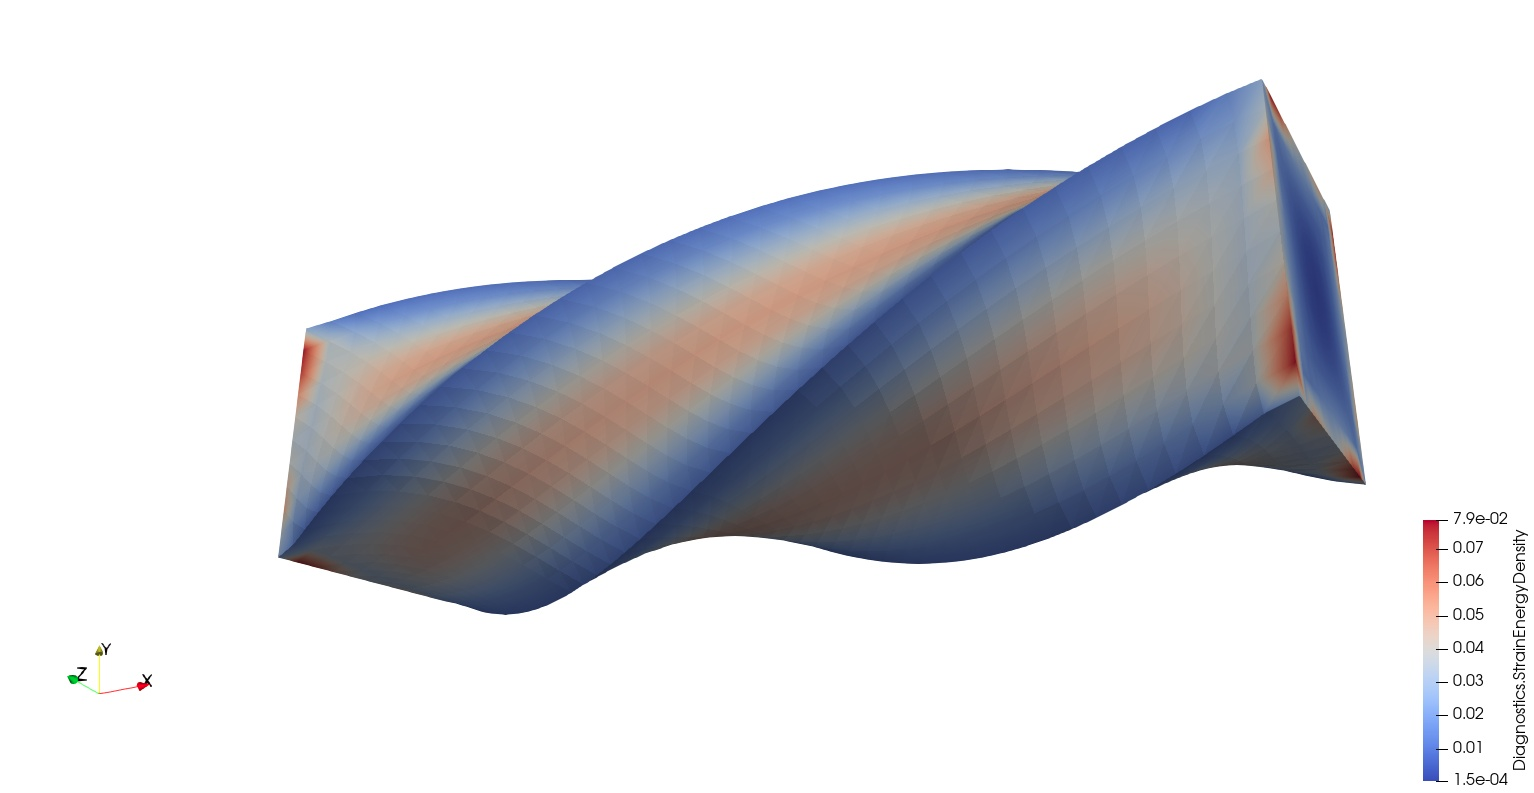
\includegraphics[height=3.2cm]{SolidTwistExample.png}
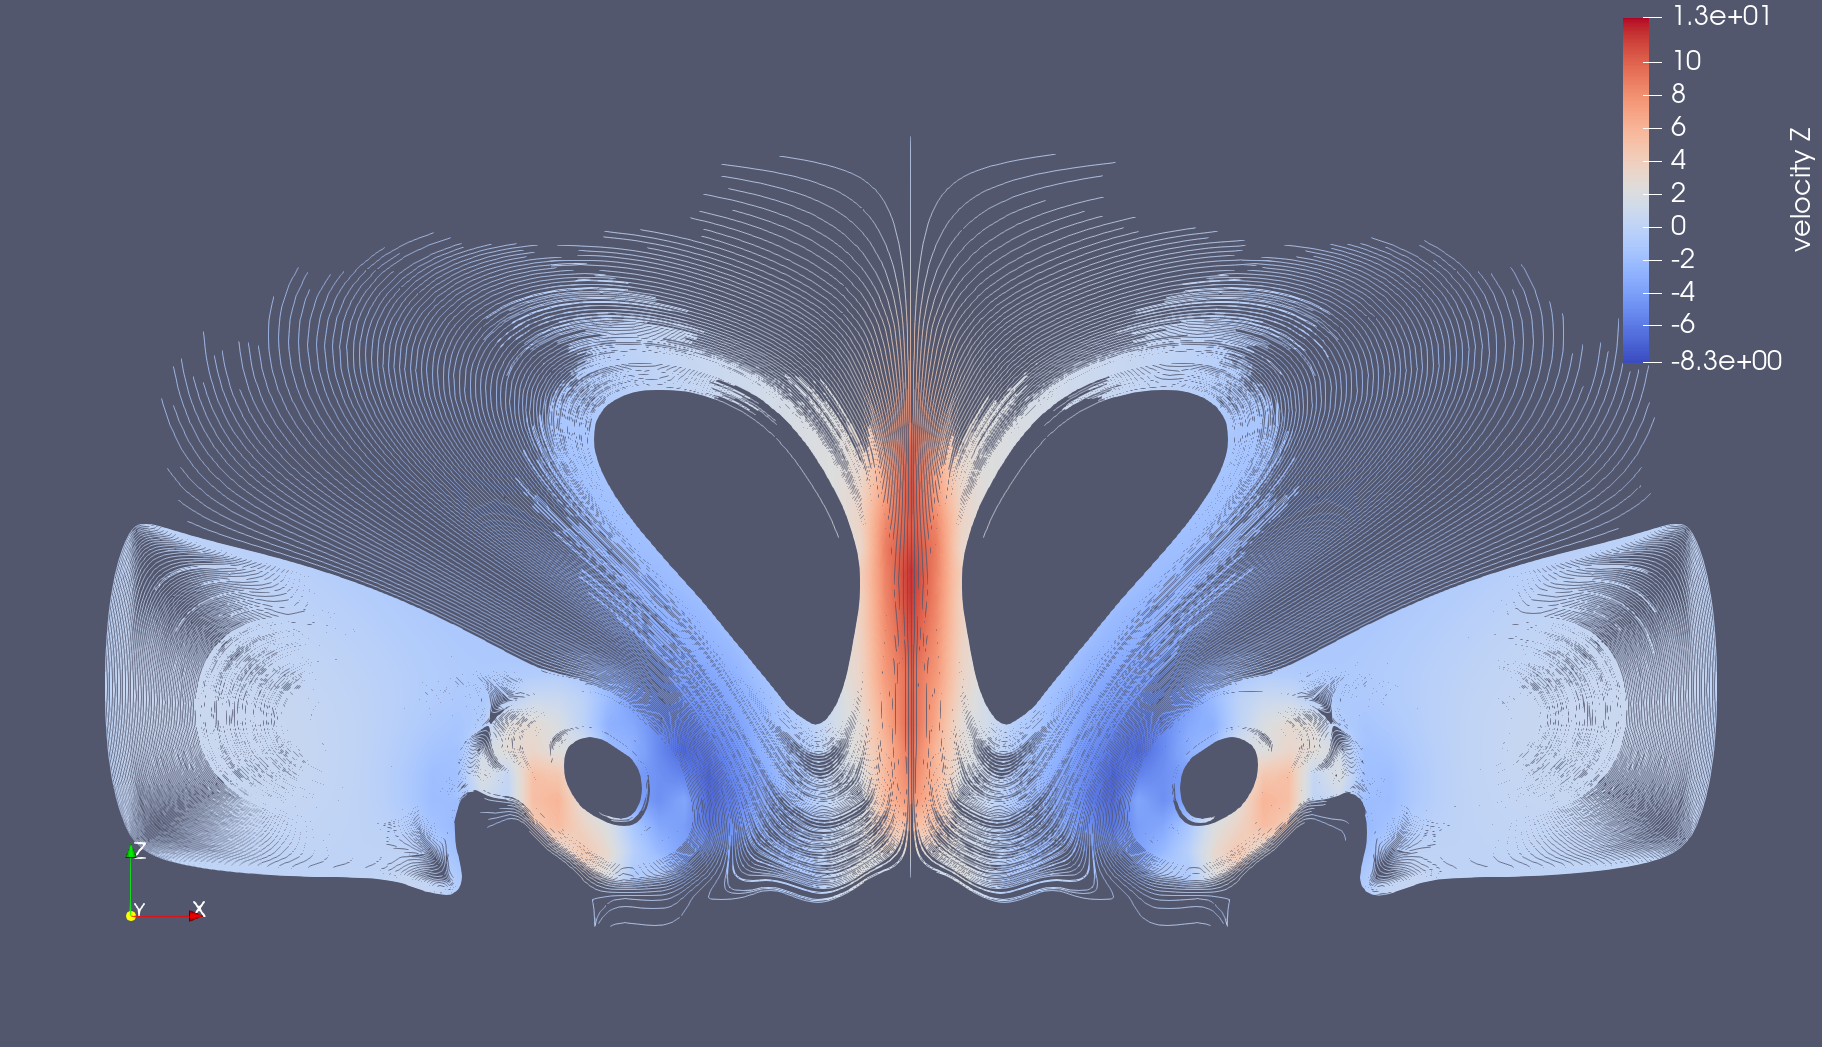
\includegraphics[height=3.2cm]{Vortices.png}

{\small libCEED solid mechanics (left) and fluid dynamics (right) mini-apps}

~\\

\begin{itemize}

\item Physics based simulations important in science/engineering

~\\

\item Intuition: FEM solves equations with piecewise polynomial solution

~\\

\item libCEED supports FEM-like simulations on modern hardware 

\end{itemize}

\end{center}
\end{frame}

%------------------------------------------------

\begin{frame}
\begin{center}
\frametitle{libCEED Projects}

Several projects built using libCEED\\

~\\

\begin{itemize}

\item Ratel - solid mechanics FEM (H1) and iMPM (PSAAP)\\

~\\

\item HONEE - fluid dynamics FEM (H1) \& differential filtering (PHASTA)\\

~\\

\item MFEM - various applications, libCEED integrators (LLNL)\\

~\\

\item Palace - Electromagnetics FEM with MFEM + libCEED (Amazon)\\
\hspace{13mm} H(div) and H(curl) elements

~\\

\item RDycore - FV river dynamical core with PETSc + libCEED (SciDAC)\\

\end{itemize}

\end{center}
\end{frame}

%------------------------------------------------

\begin{frame}
\begin{center}
\frametitle{Top 500}

\begin{table}[ht!]
\begin{center}
\begin{tabular}{l r r}
  \toprule
  Machine  &  HPL  &  HPCG  \\
  \toprule
  Fugaku     &    442.01 PFLOPs  &  16.01 PFLOPs  \\
  Frontier   &  1,353.00 PFLOPs  &  14.05 PFLOPs  \\
  Aurora     &  1,012.00 PFLOPs  &   5.61 PFLOPs  \\
  LUMI       &    379.70 PFLOPs  &   4.59 PFLOPs  \\
  Alps       &    434.90 PFLOPs  &   3.57 PFLOPs  \\
  \bottomrule
\end{tabular}
\end{center}
\end{table}
{\small Top 500 Machines for HPCG with HPL peak FLOPs}\\

~\\

Difficult to realize peak FLOPs with CG on modern machines

\end{center}
\end{frame}

%------------------------------------------------

\begin{frame}
\begin{center}
\frametitle{Modern Hardware}

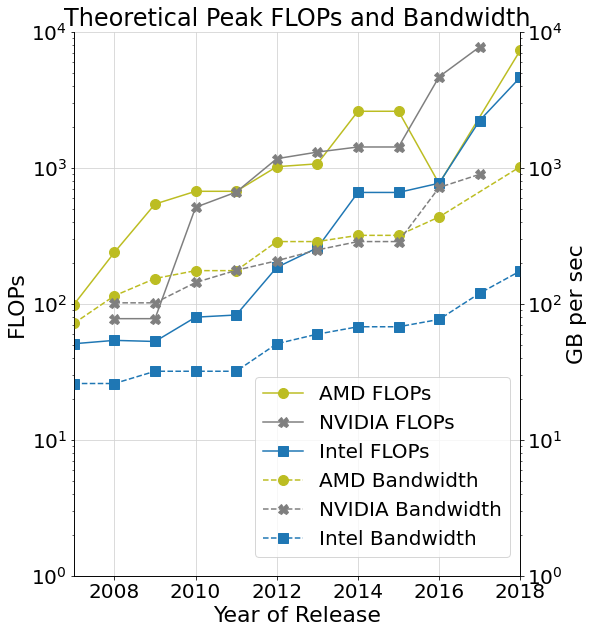
\includegraphics[height=5.5cm]{peakFlopsAndBandwidth_tall.png}
\hspace{1cm}
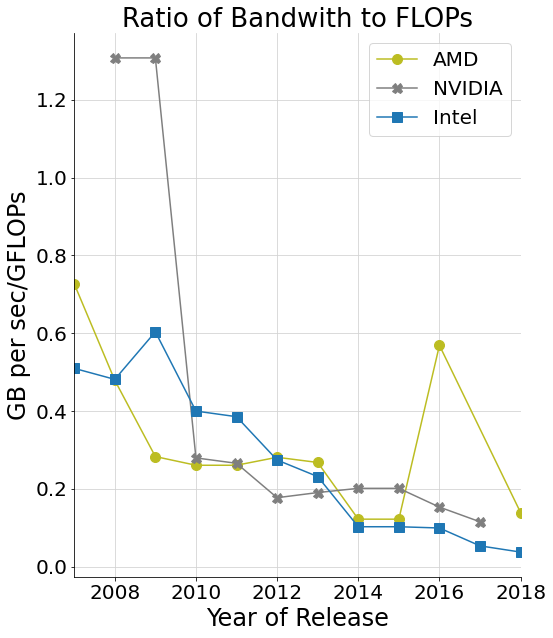
\includegraphics[height=5.5cm]{peakRatio_tall.png}

Memory bandwidth is improving slower than FLOPs \cite{kruppcomparison}\\

~\\

Mirrors difference between Top 500 HPL vs HPCG benchmarks \cite{meuertop500}\\

\end{center}
\end{frame}

%------------------------------------------------

\begin{frame}
\begin{center}
\frametitle{Matrix-Free Operators from libCEED}

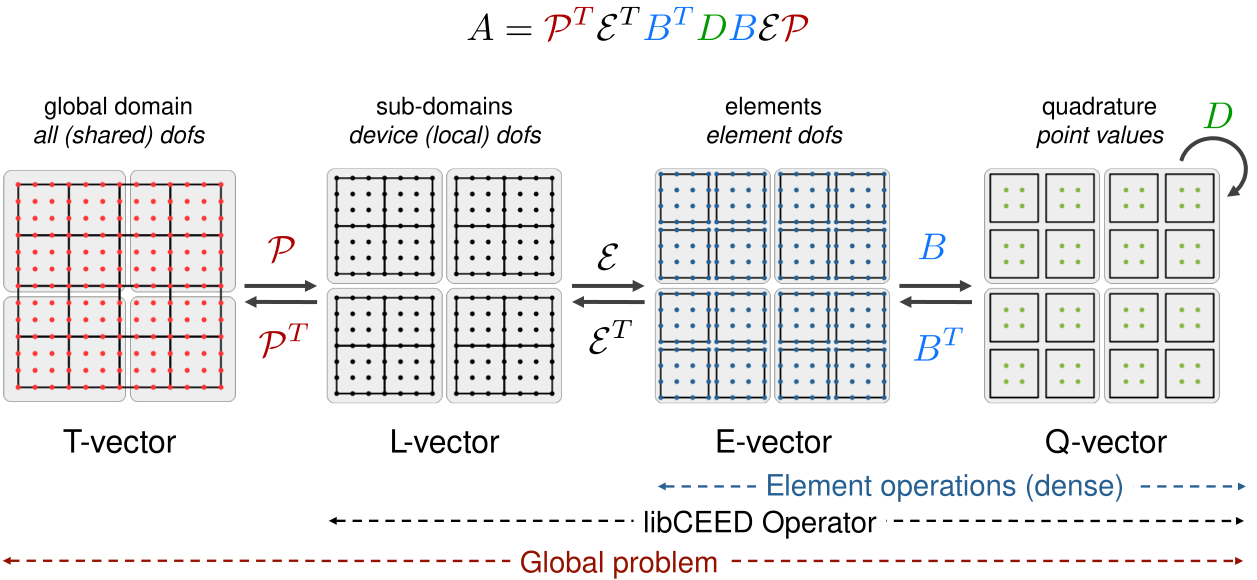
\includegraphics[height=5.0cm]{libCEEDAPI.png}

~\\

libCEED provides matrix-free operator evaluation on various hardware\\

~\\

Matrix-free operators apply these steps instead of populating a matrix\\

\end{center}
\end{frame}

%------------------------------------------------

\begin{frame}
\begin{center}
\frametitle{Benefits of Matrix-Free}

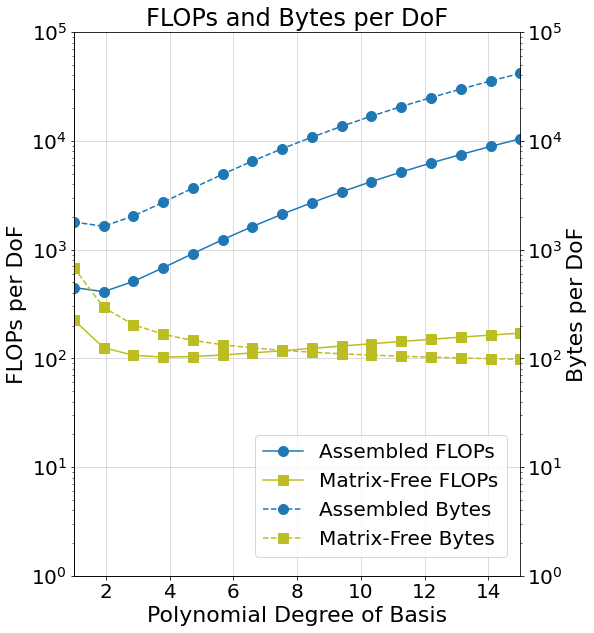
\includegraphics[height=5.5cm]{assembledVsMatrixFree_tall}
\hspace{1cm}
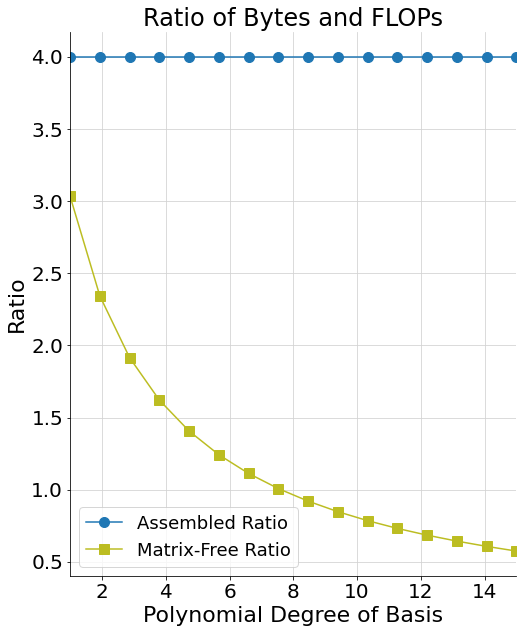
\includegraphics[height=5.5cm]{assembledVsMatrixFreeBalance_tall}

{\small Requirements for matrix-vector product with sparse matrix vs matrix-free\\ for screened Poisson $\nabla^2 u - \alpha^2 u = f$ in 3D}\\

{\bf Matrix-free representations using tensor product bases\\better match modern hardware}

\end{center}
\end{frame}

%------------------------------------------------

\begin{frame}
\begin{center}
\frametitle{Performance Portability}

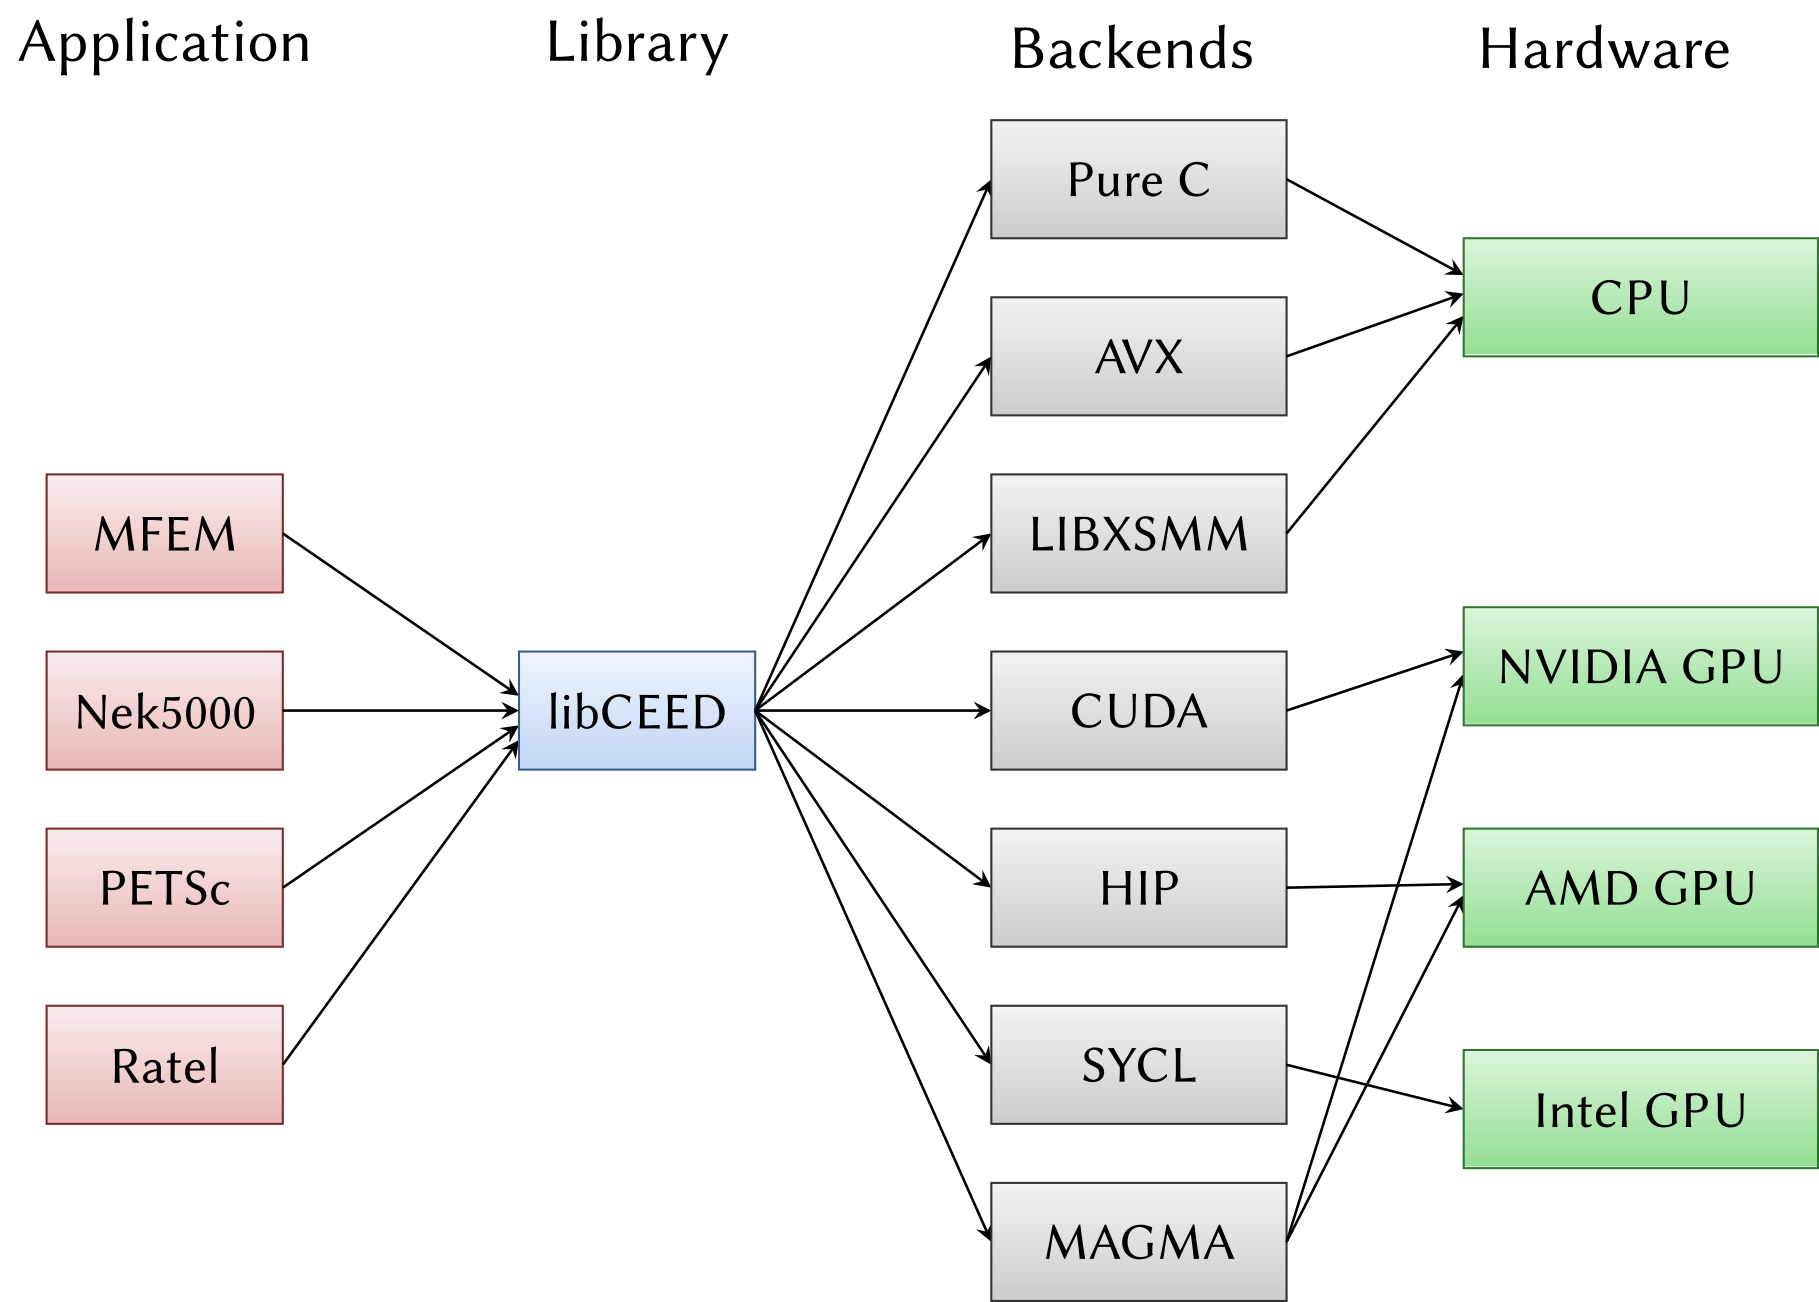
\includegraphics[height=5.5cm]{libCEEDBackends.png}

~\\

libCEED's design naturally allows multiple hardware implementations\\

\end{center}
\end{frame}

%------------------------------------------------

\begin{frame}
\begin{center}
\frametitle{Design Implications}

Using matrix-free operators drives design decisions\\

~\\

\begin{itemize}

\item Direct solvers are out (require assembled matrix)\\

~\\

\item Iterative solvers are in (Krylov methods, etc)\\

~\\

\item High order = high accuracy \& bad condition numbers\\

~\\

\item Preconditioning is needed for fast convergence\\

\end{itemize}

\end{center}
\end{frame}

%-------------------------------------------------------------------------------
\section{Ratel}
%-------------------------------------------------------------------------------

\begin{frame}
\frametitle{Ratel Team}

\begin{center}
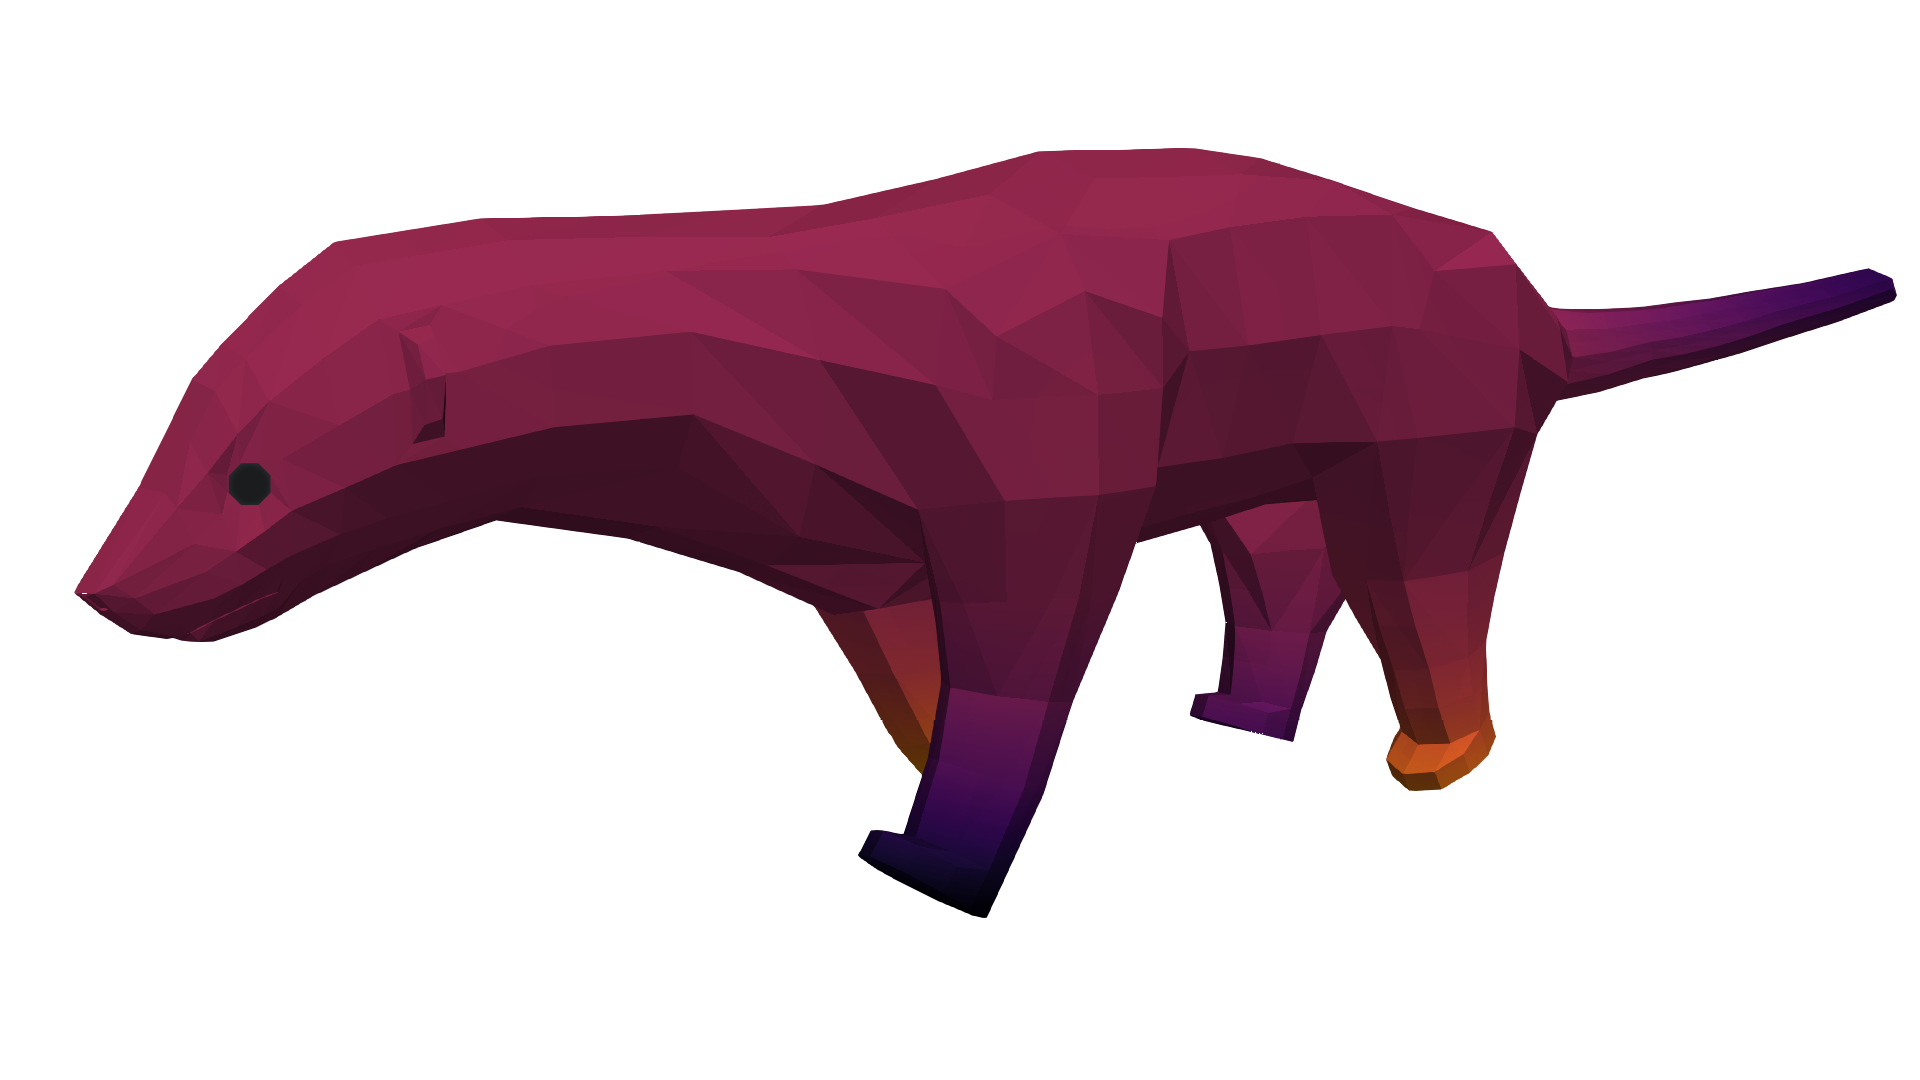
\includegraphics[height=2.75cm]{Ratellogo.png}
\end{center}

{\flushleft

Ratel Repo: \href{https://gitlab.com/micromorph/ratel}{https://gitlab.com/micromorph/ratel}\\

~\\
Developers: Zach R. Atkins, Jed Brown, Fabio Di Gioacchino,\\
\hspace{19mm} Leila Ghaffari, Zach Irwin, Rezgar Shakeri,\\
\hspace{19mm} Ren Stengel, Jeremy L Thompson\\

~\\

}

\end{frame}

%------------------------------------------------

\begin{frame}
\begin{center}
\frametitle{Basic Design}

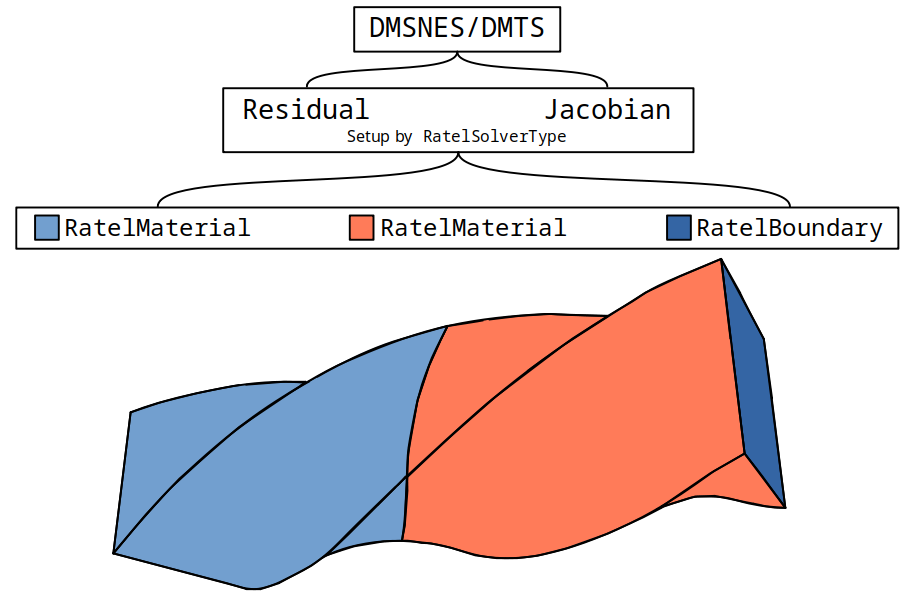
\includegraphics[height=5.5cm]{RatelAPI.png}

~\\

Each material region sets up part of the non-linear and linear equations\\

\end{center}
\end{frame}

%------------------------------------------------

\begin{frame}
\begin{center}
\frametitle{Preconditioning Support}

Iterative solvers need preconditioning, especially with high-order operators\\

~\\

\begin{itemize}

\item Jacobi - diagonal assembly\\

~\\

\item Point Block Jacobi - block diagonal assembly\\

~\\

\item Variable Point Block Jacobi - variable block diagonal assembly\\

~\\

\item Algebraic Multigrid - full assembly (best for linear elements)\\

\end{itemize}

~\\

Preconditioning support for matrix-free is an interesting research area\\

~\\

Need to balance setup costs and preconditioner effectiveness

\end{center}
\end{frame}

%------------------------------------------------

\begin{frame}
\begin{center}
\frametitle{p-multigrid}

\begin{tikzpicture}
\node[shape=circle,draw=black] (A) at (0,0) {$p_2$};
\node[shape=circle] (Al) at (-1.2,0) {Smooth};
\node[shape=circle,draw=black] (B) at (2,-2) {$p_1$};
\node[shape=circle] (Bl) at (0.8,-2) {Smooth};
\node[shape=circle,draw=black] (C) at (4,-4) {$p_0$};
\node[shape=circle] (Cl) at (4,-5) {Coarse Solve};
\node[shape=circle,draw=black] (D) at (6,-2) {$p_1$};
\node[shape=circle] (Dl) at (7.2,-2) {Smooth};
\node[shape=circle,draw=black] (E) at (8,0) {$p_2$};
\node[shape=circle] (El) at (9.2,0) {Smooth};
\path[->] (A) edge node[left=10, pos=.6] {Restriction} (B);
\path[->] (B) edge node[left=10, pos=.6] {Restriction} (C);
\path[->] (C) edge node[right=10, pos=.4] {Interpolation} (D);
\path[->] (D) edge node[right=10, pos=.4] {Interpolation} (E);
\end{tikzpicture}

\vspace{-0.9cm}

libCEED provides grid transfer operators and smoothers from operators\\

\end{center}
\end{frame}

%------------------------------------------------

\begin{frame}
\begin{center}
\frametitle{Too General, Need Specifics}

Ok, lets look at some specific simulations\\

\end{center}
\end{frame}

%------------------------------------------------

\begin{frame}[fragile]
\begin{center}
\frametitle{Example - Linear Damage}

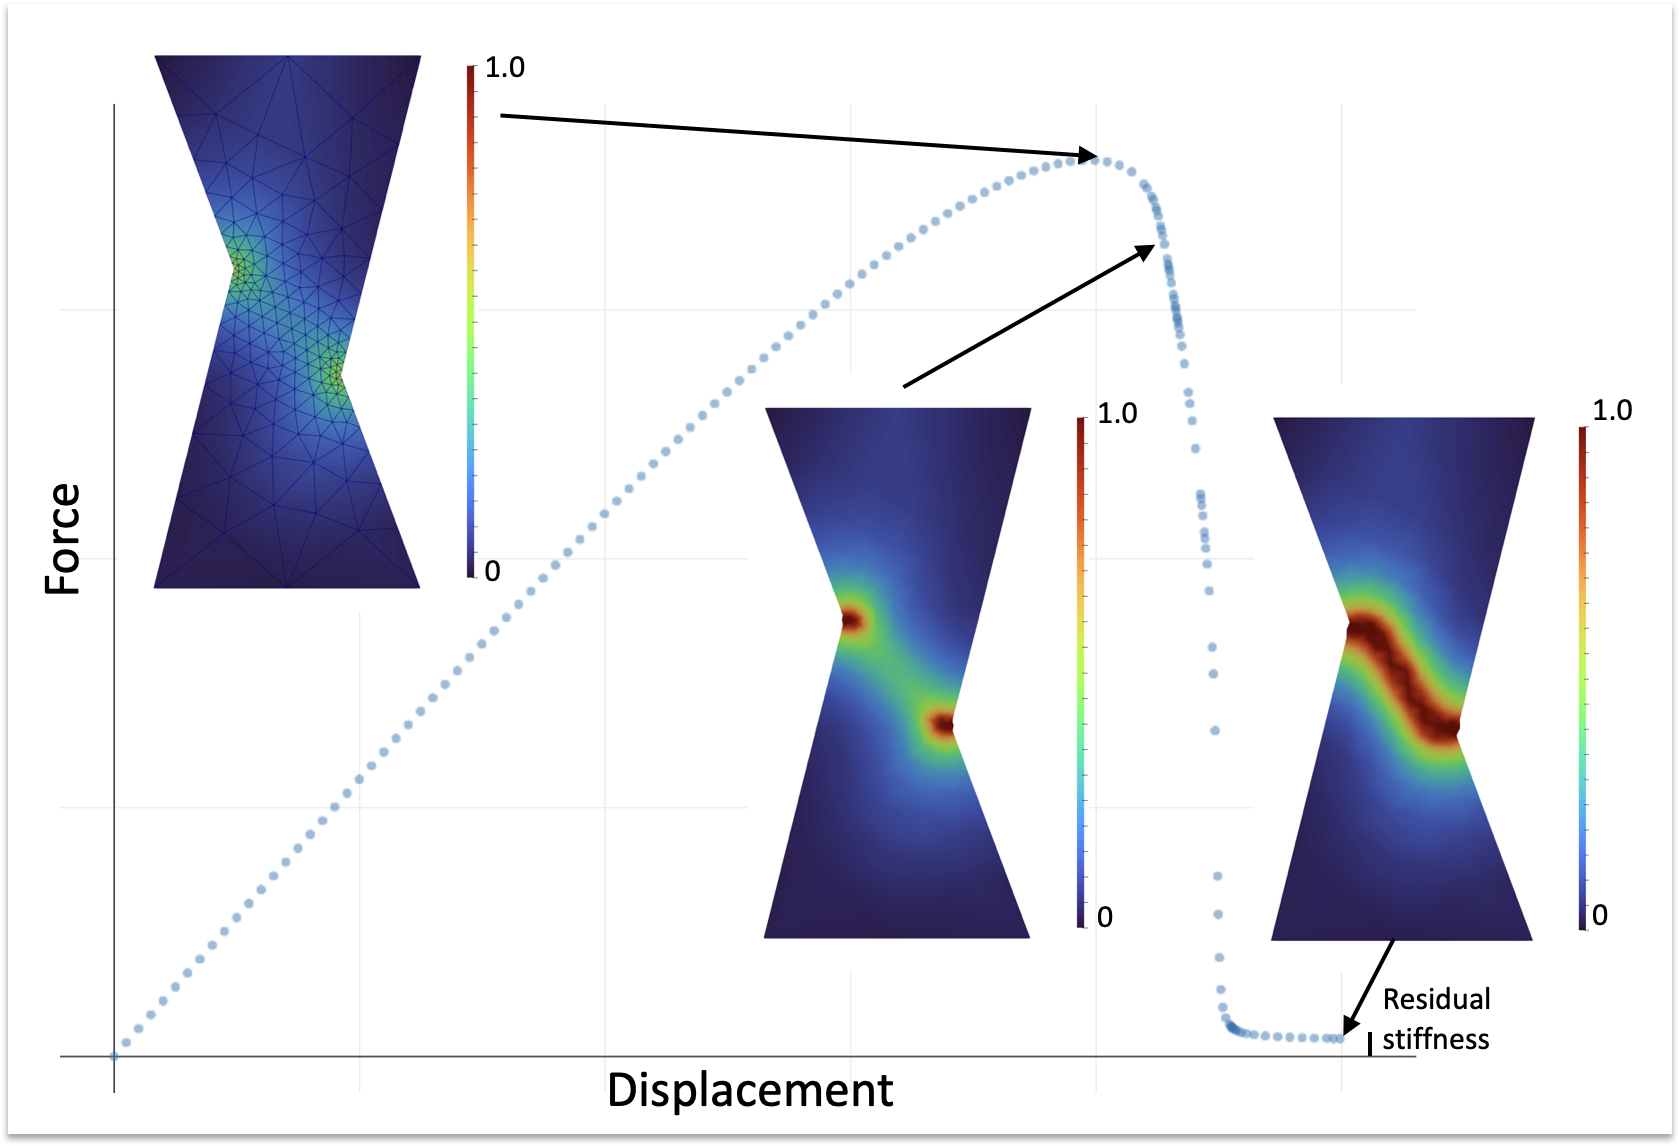
\includegraphics[height=5.0cm]{compressive-shear-damage-FEM.png}

{\tiny
\begin{lstlisting}
$ bin/ratel-quasistatic -options_file examples/ymls/ex02-quasistatic-elasticity-linear-damage-compressiveshear-AT2-face-forces.yml
\end{lstlisting}
}

Quasistatic simulation of compressive shear for generic brittle material

\end{center}
\end{frame}

%------------------------------------------------

\begin{frame}[fragile]
\begin{center}
\frametitle{Example - Dynamic Pendulum}

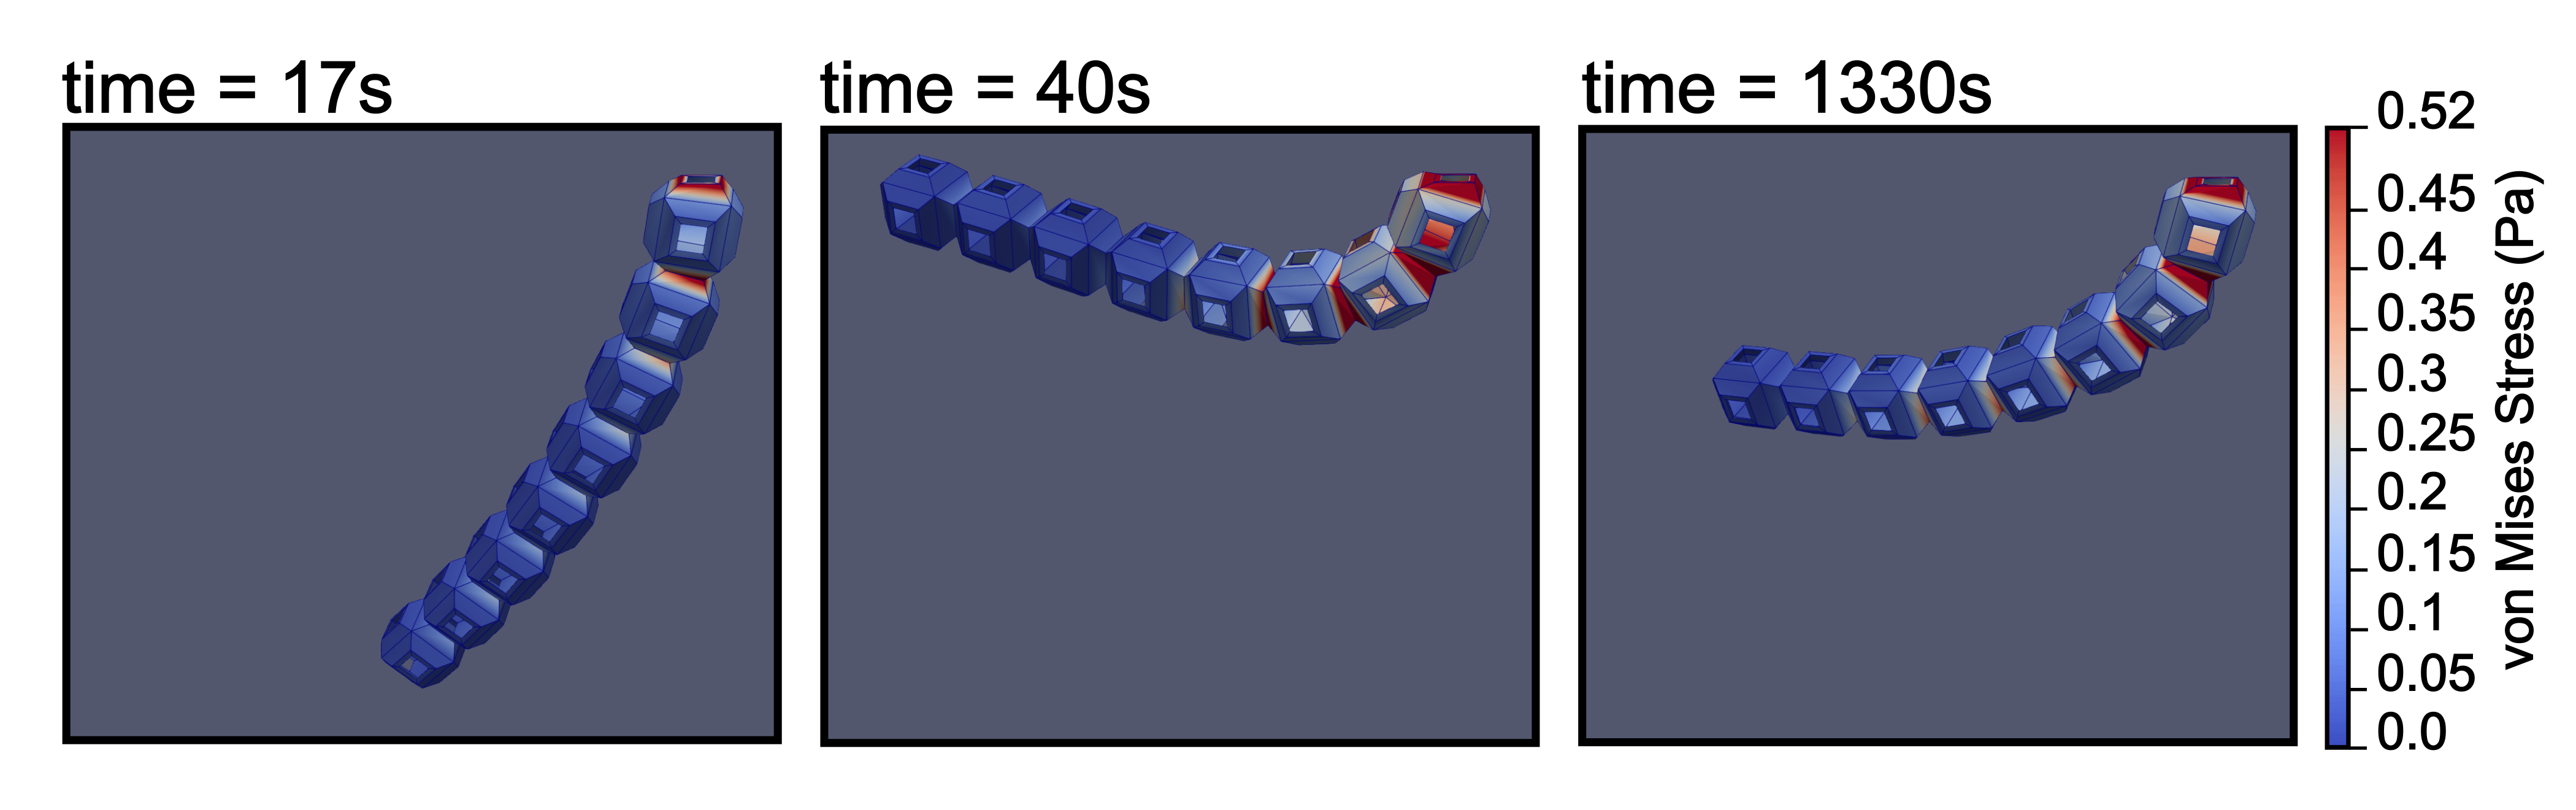
\includegraphics[height=3.8cm]{dynamic-pendulum.png}

{\tiny
\begin{lstlisting}
$ bin/ratel-dynamic -options_file examples/ymls/ex03-dynamic-elasticity-schwarz-pendulum-enzyme.yml
\end{lstlisting}
}

Dynamic simulation of Neo-Hookean Schwarz-P "pendulum" with Enzyme

\end{center}
\end{frame}

%------------------------------------------------

\begin{frame}
\begin{center}
\frametitle{What is MPM?}

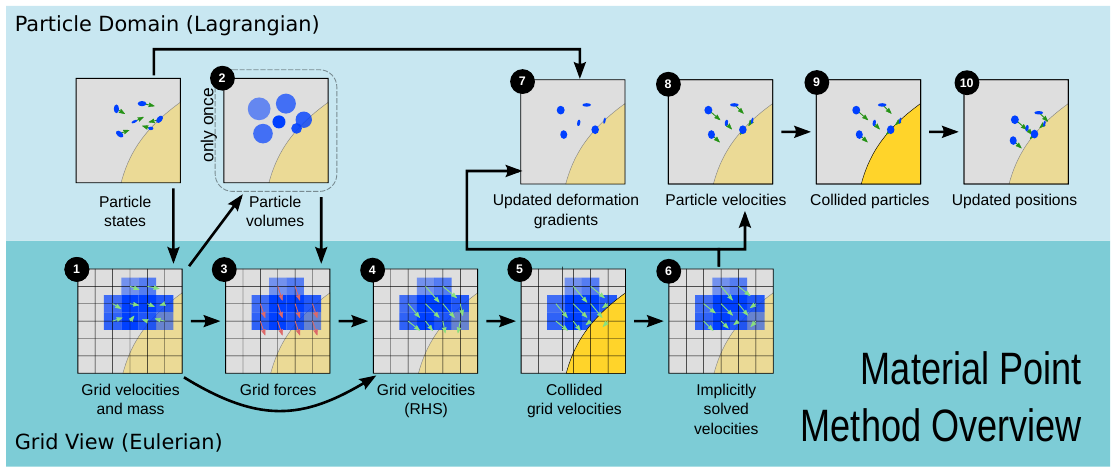
\includegraphics[height=5cm]{MPMOverview.png}\\

~\\

\begin{itemize}

\item Continuum based particle method with background mesh for gradients\\

\item Extension of FLIP (which is an extension of PIC)\\

\item Used in rendering for the movie \emph{Frozen}\\

\end{itemize}

\end{center}
\end{frame}

%------------------------------------------------

\begin{frame}[fragile]
\begin{center}
\frametitle{Example - MPM Sinker}

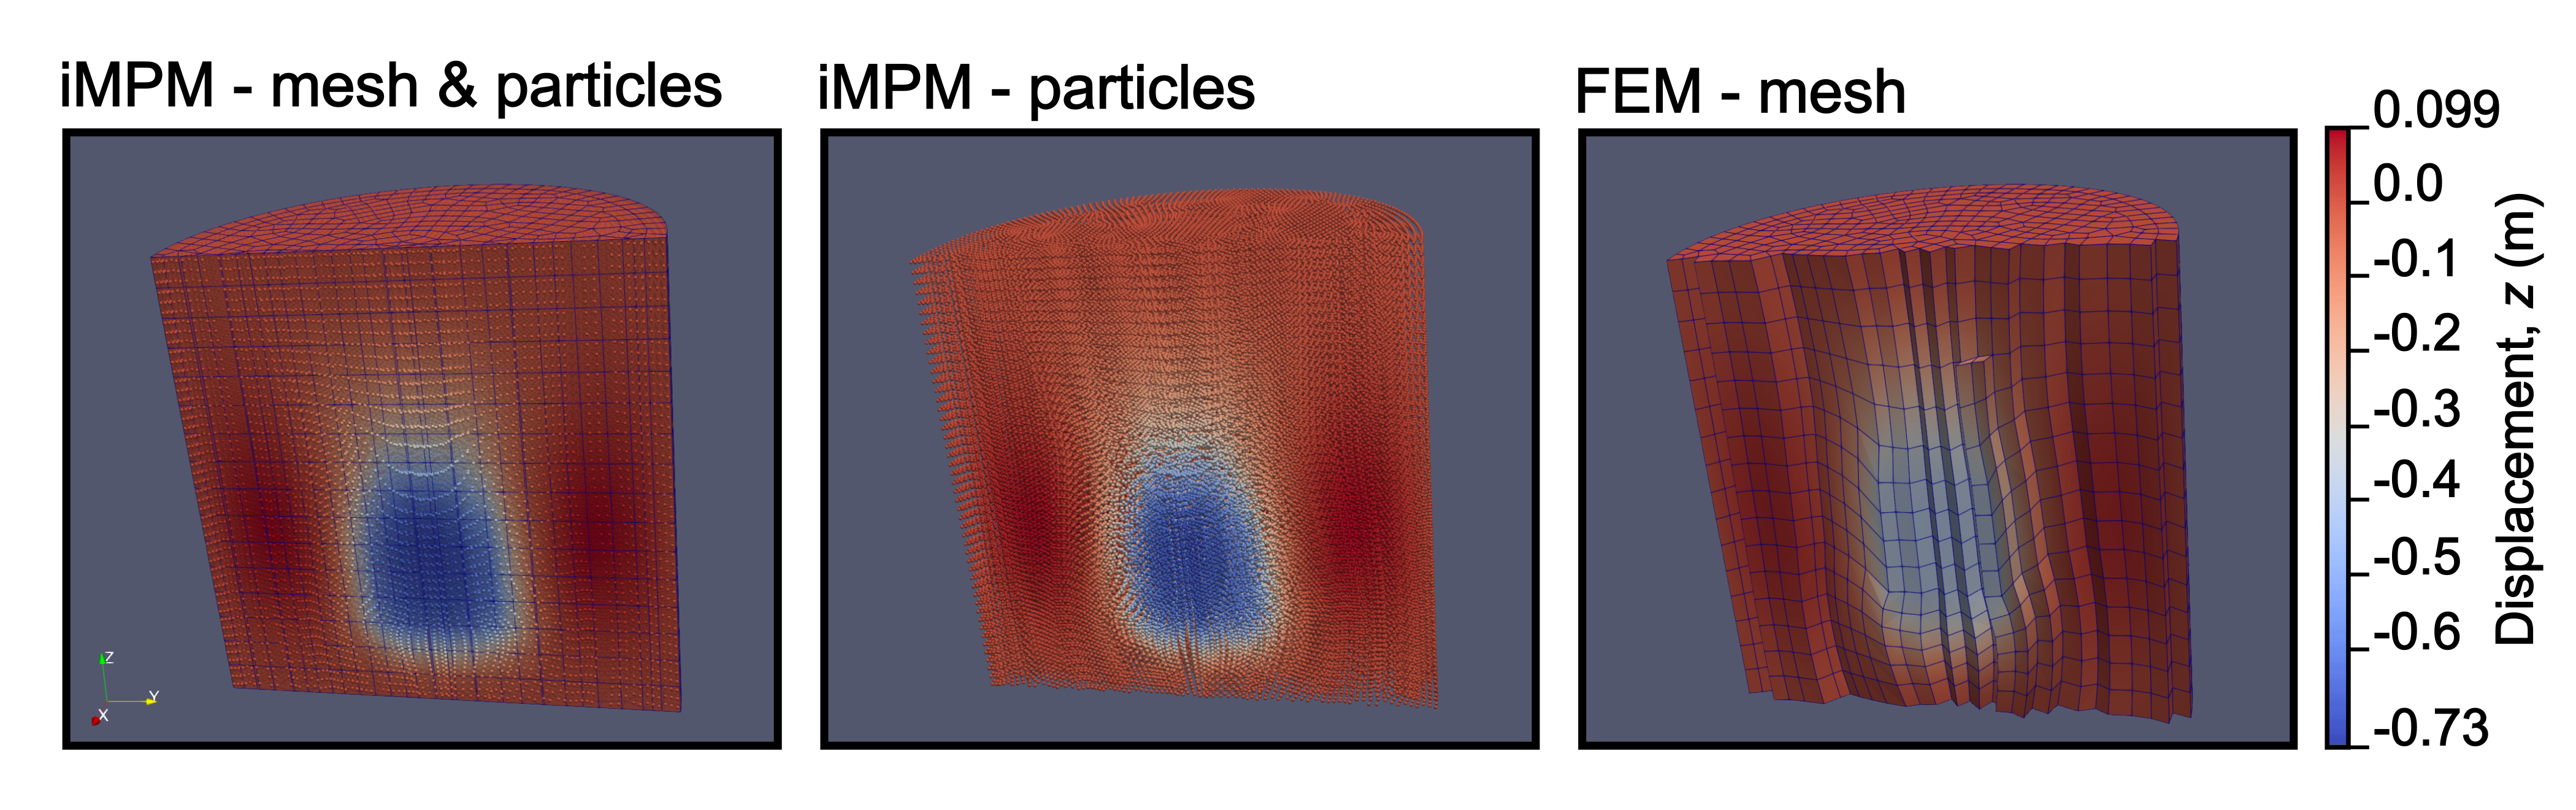
\includegraphics[height=3.8cm]{sinker-MPM-FEM.png}

{\tiny
\begin{lstlisting}
$ bin/ratel-quasistatic -options_file examples/ymls/ex02-quasistatic-elasticity-mpm-neo-hookean-damage-current-sinker-cylinder.yml
\end{lstlisting}
}

FEM and iMPM simulations of dense sinker in near-incompressible "foam"

\end{center}
\end{frame}

%-------------------------------------------------------------------------------
\section{Mentoring}
%-------------------------------------------------------------------------------

\begin{frame}
\begin{center}
\frametitle{Dev Best Practices}

Open Source development best practices provide mentoring framework\\

~\\

\begin{itemize}

\item Issues/planning act as literature review/research plan

~\\

\item PR/MRs provide feedback about the work

~\\

\item Testing verifies correctness, to a degree

~\\

\item Documentation gives an opportunity to show understanding 

\end{itemize}

\end{center}
\end{frame}

%------------------------------------------------

\begin{frame}
\begin{center}
\frametitle{Planning}

Planning establishes common understanding and goals

~\\

\begin{itemize}

\item Codebases can easily overwhelm new students/contributors

~\\

\item Issues help focus the effort and coalesce conversations

~\\

\item Planning publicly (Issues ideally, or Slack/Zulip) records decisions

~\\

\item Good example: \href{https://gitlab.com/micromorph/ratel/issues/270}{https://gitlab.com/micromorph/ratel/issues/270}\\

\end{itemize}

\end{center}
\end{frame}

%------------------------------------------------

\begin{frame}
\begin{center}
\frametitle{Review}

Code review provides feedback and discussions

~\\

\begin{itemize}

\item All code can be strengthened with review and feedback

~\\

\item PR/MRs provide tangible assets to guide any discussion

~\\

\item Public review lets multiple people comment; prevents surprises

~\\

\item Easy to be more/less explicit as appropriate for the student

\end{itemize}

\end{center}
\end{frame}

%------------------------------------------------

\begin{frame}
\begin{center}
\frametitle{Testing}

Testing is as essential part of MR acceptance

~\\

\begin{itemize}

\item Tests communicate intended usage and verify correctness

~\\

\item New logic must have tests, code coverage is a \textbf{guide}

~\\

\item Minimal reproducers for bugs also make good tests

~\\

\item Untested code is broken code; tested code is less broken code\\

\end{itemize}

\end{center}
\end{frame}

%------------------------------------------------

\begin{frame}
\begin{center}
\frametitle{Documentation}

Documentation ensures understanding and maintainability

~\\

\begin{itemize}

\item Code needs documentation

~\\

\item Another avenue to communicate/verify understanding

~\\

\item Documentation can also be used to start papers/dissertations

~\\

\item Good documentation facilitates planning for new features

\end{itemize}

\end{center}
\end{frame}

%-------------------------------------------------------------------------------
\section{Questions}
%-------------------------------------------------------------------------------

\begin{frame}
\frametitle{Questions?}

\begin{center}
\includegraphics[height=2.75cm]{libCEEDlogo.png}
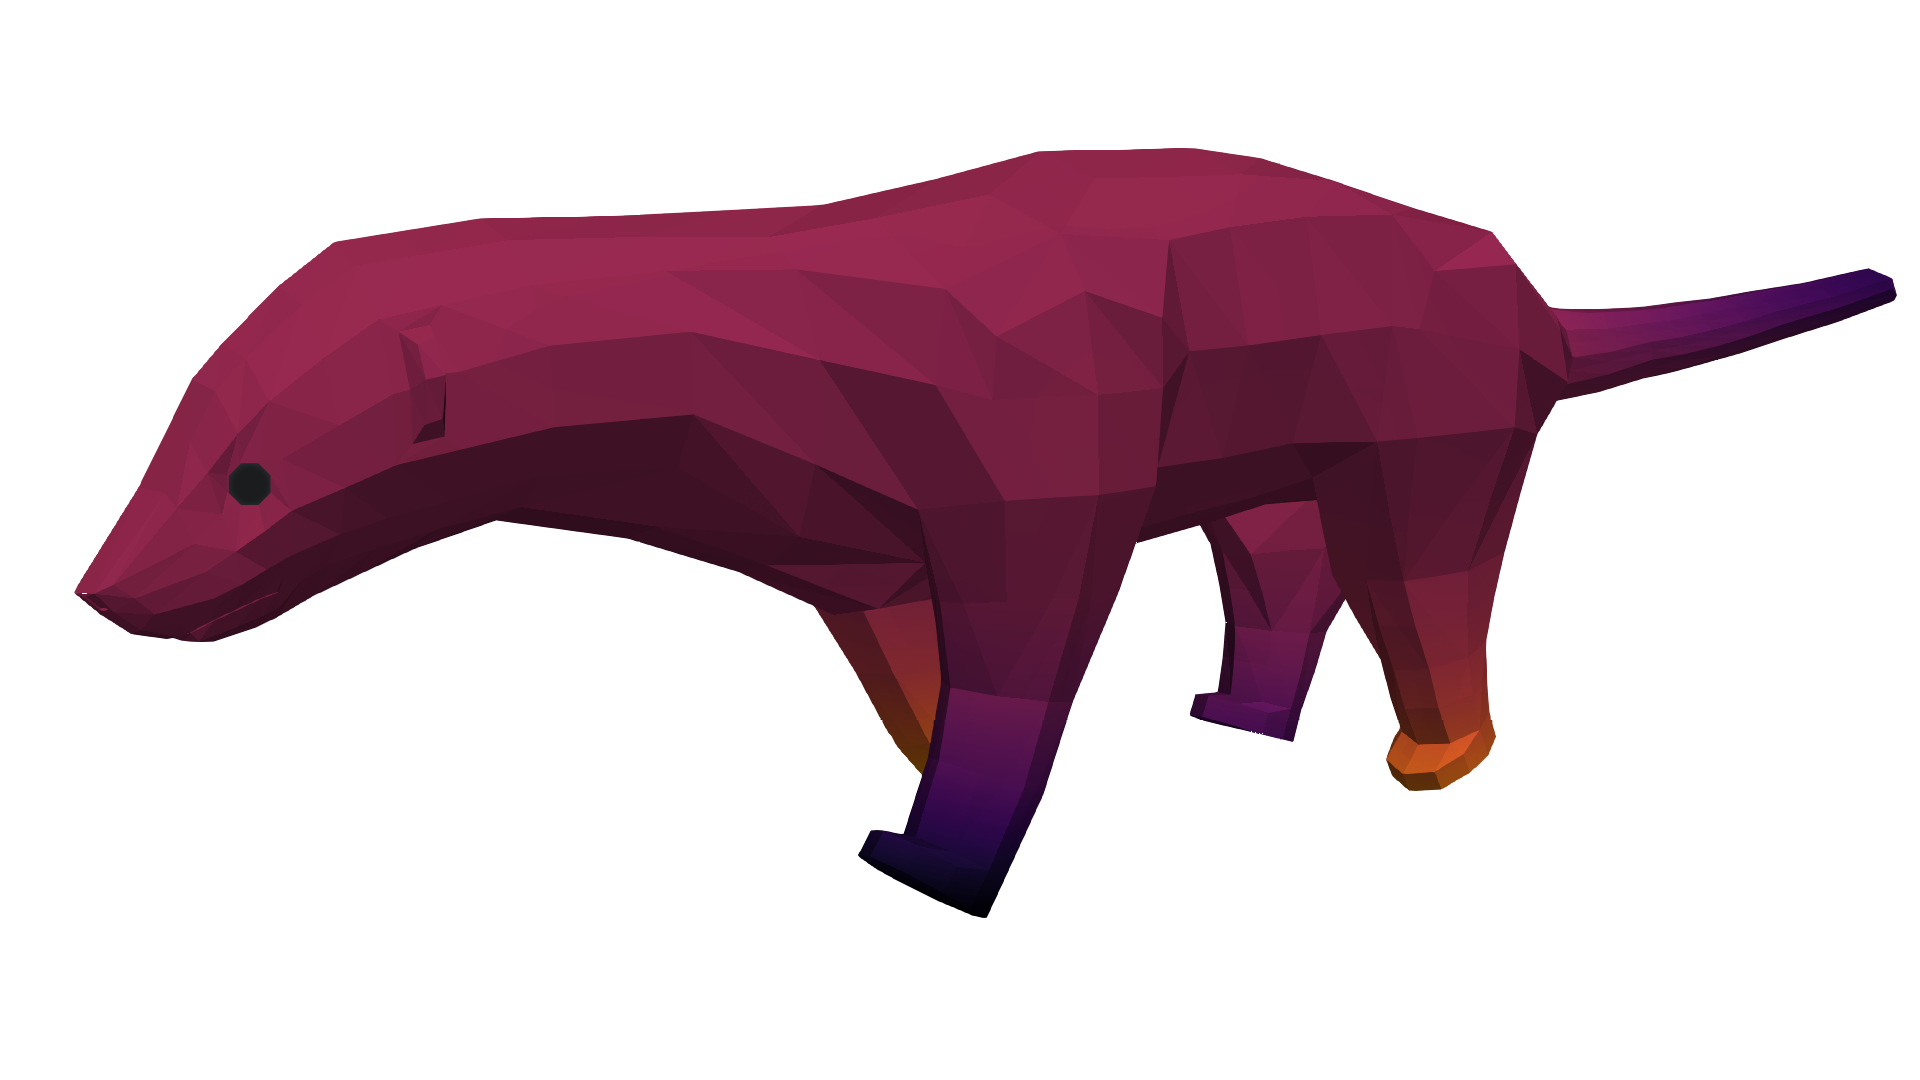
\includegraphics[height=2.75cm]{Ratellogo.png}
\end{center}

{\flushleft

libCEED Repo: https://github.com/CEED/libCEED\\
Ratel Repo: https://gitlab.com/micromorph/ratel\\

~\\

Grant: Predictive Science Academic Alliance Program (DE-NA0003962)\\

}

\begin{center}

\includegraphics[height=0.8cm]{psaap-center-logos.png}
\end{center}

\end{frame}

%-------------------------------------------------------------------------------

\begin{frame}[noframenumbering]
\titlepage % Print the title page
\end{frame}

\begin{frame}[noframenumbering,allowframebreaks]
\bibliographystyle{plain}  % or "siam", or "alpha", etc.
\bibliography{references}  % Bib database in "refs.bib"
\end{frame}

\begin{frame}[noframenumbering]
\titlepage % Print the title page
\end{frame}

%-------------------------------------------------------------------------------

\end{document}

%-------------------------------------------------------------------------------
